\chapter{実験原理}
\label{apparatus}

%\section{概要}

この章では本研究で用いた実験装置,
及び新しい装置の製作と,
新たに導入したトリガー用のプラスチックシンチレータ(以下SCtrig)の評価,
磁場中におけるPMTの動作確認について述べる.
%この章では本研究で用いた実験装置,
%及び今後の研究で導入予定のトリガー用のプラスチックシンチレータ(以下SCtrig)の評価と,
%実験装置の改良について述べる.


\section{寿命測定}

ポジトロニウムを形成するために使用する線源は$\mathrm{^{22}Na}$である.
$\mathrm{^{22}Na}$は,半減期が2.602 年であり,
$\beta^{+}$崩壊(式\ref{eq:beta}),電子捕獲により,$\mathrm{^{22}Ne}$になる.
この$Q$値は2842 keVである.\cite{ToRI}
また$\beta^{+}$崩壊をしてできた励起状態の$\mathrm{^{22}Ne}$は,
1275 keVの$\gamma$線を放出し,基底状態の$\mathrm{^{22}Ne}$となる.(図\ref{fig:na})

\begin{equation}
\mathrm{^{22}Na} \to \mathrm{^{22}Ne} + \mathrm{e^{+}} + \nu_{\mathrm{e}}
\label{eq:beta}
\end{equation}

\begin{figure}[H]
\centering
\includegraphics[keepaspectratio,scale=0.4]{fig/ybm/na.pdf}
\caption{$\mathrm{^{22}Na}$の崩壊\cite{ToI}}
\label{fig:na}
\end{figure}

昨年度までの研究では,トリガーとして1275 keVの$\gamma$線を使用していたが,
本研究では,陽電子がSCtrigを通過した信号をトリガーとして用いるための装置を製作した.
トリガー信号と,ポジトロニウムが崩壊し放出される$\gamma$線が検出された時間差を測定することで,
寿命を計算する.
ポジトロニウムの寿命$\tau$は
\begin{equation}
N(t) = N_{0} \exp( - \frac{t}{\tau})
\label{eq:lifefit}
\end{equation}
で定義される.
実験で得られた崩壊時間分布のヒストグラムを式(\ref{eq:lifefit})でフィッティングし,
寿命を得る.


\section{実験装置}

\subsection{セットアップ(担当:宮辺)}

本実験ではトリガーの1.275 MeVと,
ポジトロニウムの崩壊による$\gamma$線を検出するために,
SCIONIX製のNaI(Tl)シンチレータ(図\ref{fig:naitl})と,
浜松ホトニクス製の光電子増倍管アッセンブリH6410(図\ref{fig:pmtbig})を使用する.
NaI(Tl)シンチレータは,直径57 mm,長さ58 mmの円筒形であり,
PMT H6410の管径は直径60 mm,長さが200 mm,
ダイノード構造はラインフォーカス型である.

\begin{figure}[htbp]
\begin{minipage}{0.5\hsize}
\centering
\includegraphics[keepaspectratio,scale=0.35]{fig/ybm/naitl.pdf}
\caption{NaI(Tl)シンチレータ}
\label{fig:naitl}
\end{minipage}
\begin{minipage}{0.5\hsize}
\centering
\includegraphics[keepaspectratio,scale=0.35]{fig/ybm/naitl0.pdf}
	\caption{NaI(Tl)シンチレータの概要図\cite{nai}}
\label{fig:naitl0}
\end{minipage}
\end{figure}

また製作した実験装置では,
トリガーに用いるSCtrigから出た光を検出するために,
浜松ホトニクス製の光電子増倍管アッセンブリR2248(図\ref{fig:pmtmini})を使用する.
PMT R2248の管径は9.8mm $\times$ 9.8mmの四角で,ソケットを含めた長さは100 mm,
ダイノード構造はラインフォーカス型である.
PMTは完全な暗中にあるときでも微小な電流を出力している.
これを暗電流といい,測定する前にPMTを数十分程度暗中に放置することで減少させることができる.
トリガーに陽電子を用いることで,
陽電子がシリカエアロゲルに到達し,ポジトロニウムを形成していることを確かめ,
またSCtrigに取り付けた2本のPMTによる同時計測により,
暗電流のレートを減らし,バックグラウンドを低減させることが,SCtrigを導入する目的である.

\begin{figure}[htbp]
\begin{minipage}{0.5\hsize}
\centering
\includegraphics[keepaspectratio,angle=90,scale=0.4]{fig/ybm/pmtmini.pdf}
	\caption{PMT R2248の外形寸法図\cite{pmtshape}}
\label{fig:pmtmini}
\end{minipage}
\begin{minipage}{0.5\hsize}
\centering
\includegraphics[keepaspectratio,angle=90,scale=0.4]{fig/ybm/pmtbig.pdf}
	\caption{PMT H6410の外形寸法図\cite{pmtshape}}
\label{fig:pmtbig}
\end{minipage}
\end{figure}

またポジトロニウムに磁場をかけるために図\ref{fig:mag},\ref{fig:magnet}のような電磁石を使用する.
コイルの直径は370 mm,コイル間の距離は185 mm,
磁極の直径は100 mm,磁極間の距離は150 mmである.

定格6.0 Aの電流で,0.1 Tの磁場がかかる.
ここで\ref{fig:magnet}のように,
$z$,$\theta$方向を定義し,
$z=0$を磁極間中心に,$\theta=0$を水平方向にとる.


\begin{figure}[H]
\centering
\includegraphics[keepaspectratio,angle=90,scale=0.4]{fig/ybm/mag.pdf}
\caption{電磁石}
\label{fig:mag}
\end{figure}

\begin{figure}[H]
\centering
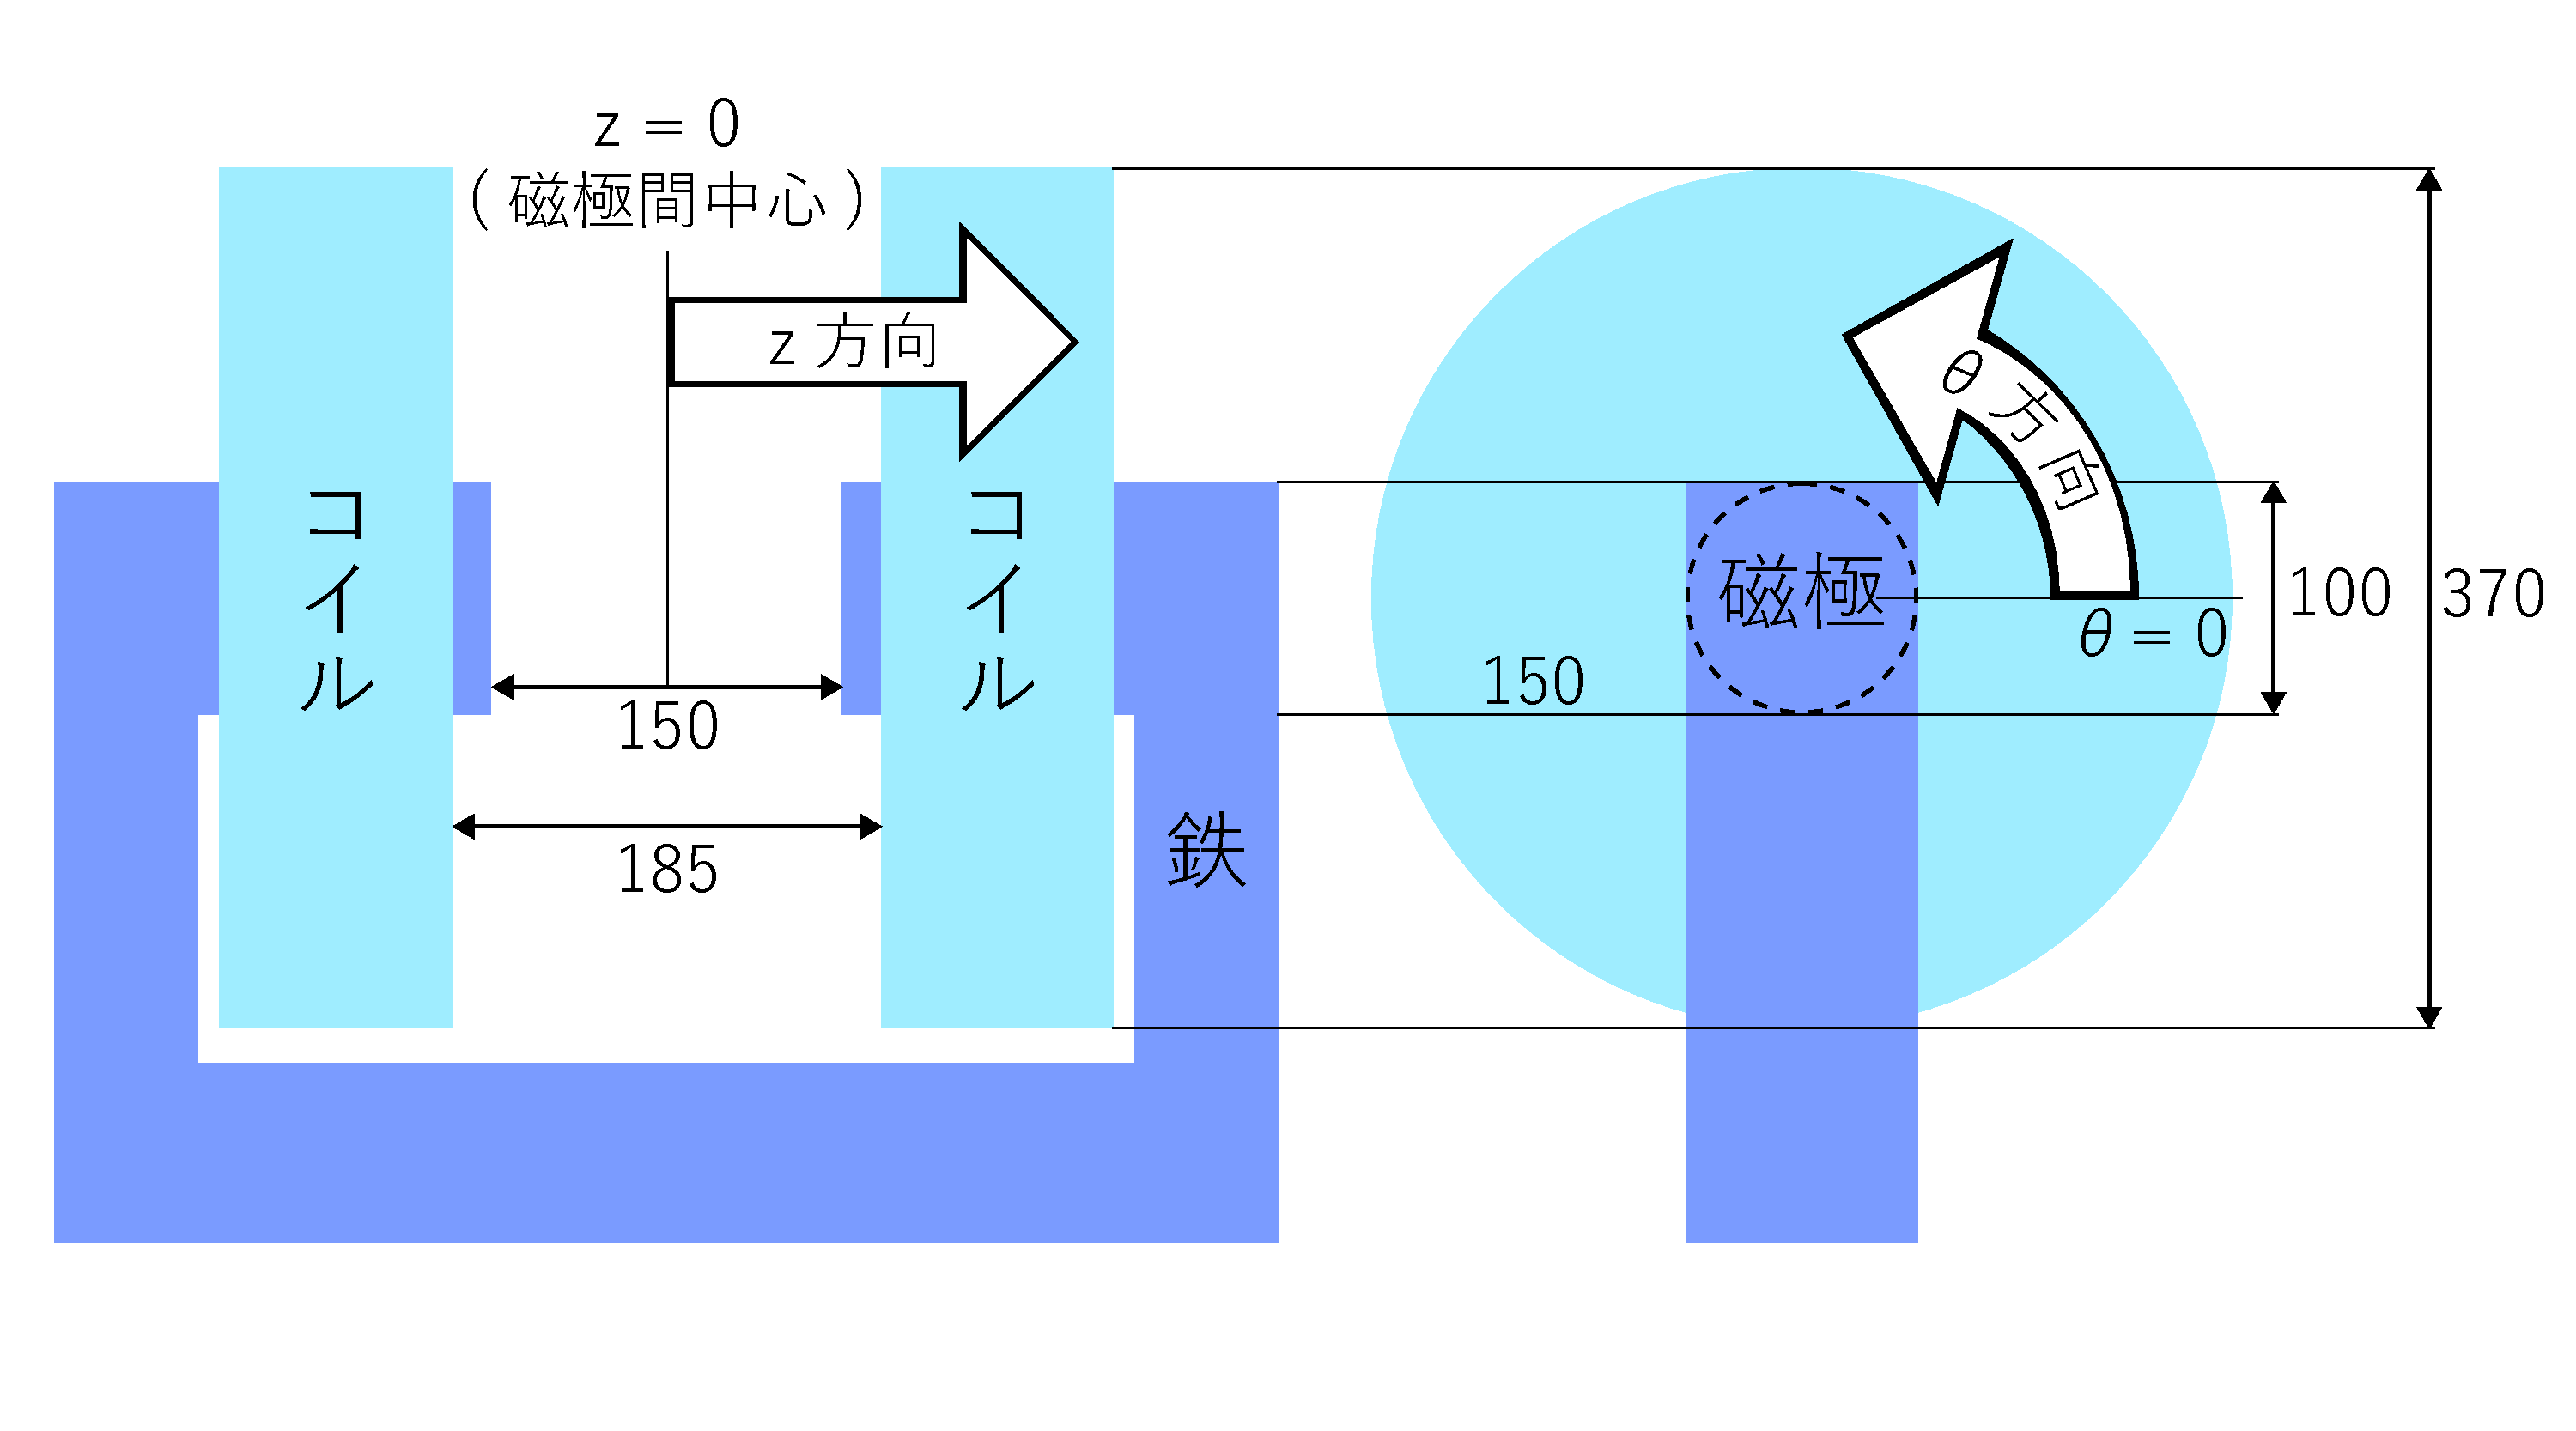
\includegraphics[keepaspectratio,scale=0.25]{fig/ybm/magnet.pdf}
\caption{電磁石の概要図}
\label{fig:magnet}
\end{figure}

本実験で使用した装置は図\ref{fig:device5},\ref{fig:device6}のようなものである,
$\mathrm{^{22}Na}$線源から出る1275 keVの$\gamma$線を,
上部に置いたNaI(Tl)シンチレータとPMT H6410で検出しトリガーとする.
陽電子はコリメータを通り,
プラスチック容器中のシリカエアロゲルでポジトロニウムを形成する.
ポジトロニウムが崩壊し放出された$\gamma$線は,
$120^{\circ}$の角度に置かれた3つのNaI(Tl)シンチレータとPMT H6410で検出される.

\begin{figure}[H]
\begin{minipage}{0.5\hsize}
\centering
\includegraphics[keepaspectratio,scale=0.3]{fig/ybm/device5.pdf}
\caption{横から見た実験装置の概要図}
\label{fig:device5}
\end{minipage}
\begin{minipage}{0.5\hsize}
\centering
\includegraphics[keepaspectratio,scale=0.3]{fig/ybm/device6.pdf}
\caption{上から見た実験装置の概要図}
\label{fig:device6}
\end{minipage}
\end{figure}

製作した実験装置は図\ref{fig:device2},\ref{fig:device3},
トリガー部分は図\ref{fig:device3}のようになる.
$\mathrm{^{22}Na}$線源からの陽電子がコリメータを通り,SCtrigを通過し,
真空容器中のシリカエアロゲルでポジトロニウムを形成する.
SCtrigから出る光子はアクリルライトガイドを通り,
アクリルライトガイドに取り付けた2本のPMT R2248で同時計測し,
ポジトロニウムが崩壊し放出された$\gamma$線は,

$\theta=45^{\circ},135^{\circ},225^{\circ},315^{\circ}$に
4つ置かれたNaI(Tl)シンチレータとPMT H6410で検出される.
後に詳しく述べるが,すべてのPMTは磁場を遮蔽するための鉄管の中に入っている.


\begin{figure}[H]
\begin{minipage}{0.5\hsize}
\centering
\includegraphics[keepaspectratio,scale=0.3]{fig/ybm/device2.pdf}
\caption{z方向から見た実験装置の概要図}
\label{fig:device2}
\end{minipage}
\begin{minipage}{0.5\hsize}
\centering
\includegraphics[keepaspectratio,scale=0.3]{fig/ybm/device3.pdf}
\caption{実験装置の磁極間の概要図}
\label{fig:device3}
\end{minipage}
\end{figure}

\begin{figure}[H]
\centering
\includegraphics[keepaspectratio,scale=0.4]{fig/ybm/device4.pdf}
\caption{トリガー部分の概要図}
\label{fig:device3}
\end{figure}

